\documentclass{standalone}
\usepackage{tikz}
\usetikzlibrary{shapes.geometric, positioning}

\begin{document}
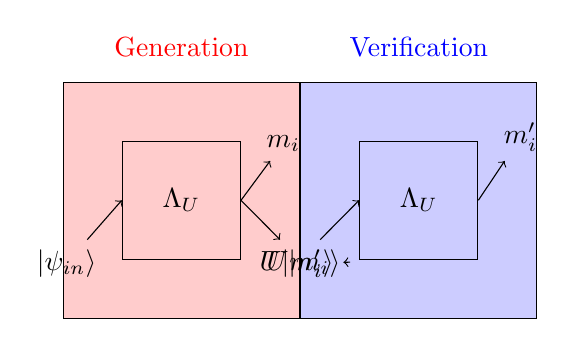
\begin{tikzpicture}

% Colors
\definecolor{lightred}{rgb}{1,0.8,0.8}
\definecolor{lightblue}{rgb}{0.8,0.8,1}

% Nodes
\node[draw, rectangle, fill=lightred, minimum width=3cm, minimum height=3cm] (gen) {};
\node[draw, rectangle, fill=lightblue, right=0cm of gen, minimum width=3cm, minimum height=3cm] (ver) {};

% Generation block
\node[draw, rectangle, minimum width=1.5cm, minimum height=1.5cm] at (gen) (genblock) {$\Lambda_U$};
\node[below left=0.5cm and 0.2cm of genblock.west] (psiin) {$|\psi_{\text{in}}\rangle$};
\node[above right=0.5cm and 0.2cm of genblock.east] (mi) {$m_i$};
\node[below right=0.5cm and 0.2cm of genblock.east] (umi) {$U |m_i\rangle$};

% Arrows for generation
\draw[->] (psiin) -- (genblock.west);
\draw[->] (genblock.east) -- (mi);
\draw[->] (genblock.east) -- (umi);

% Verification block
\node[draw, rectangle, minimum width=1.5cm, minimum height=1.5cm] at (ver) (verblock) {$\Lambda_U$};
\node[below left=0.5cm and 0.2cm of verblock.west] (umi_ver) {$U |m'_i\rangle$};
\node[above right=0.5cm and 0.2cm of verblock.east] (miprime) {$m'_i$};

% Arrows for verification
\draw[->] (umi) -- (umi_ver);
\draw[->] (verblock.east) -- (miprime);
\draw[->] (umi_ver) -- (verblock.west);

% Labels
\node[above=0.2cm of gen.north, red] {Generation};
\node[above=0.2cm of ver.north, blue] {Verification};

\end{tikzpicture}
\end{document}